The CBGB apparatus design is separated by various stages, from a room temperature 300K outer aluminum vacuum can, a nominally 40K aluminum radiation shield, and an inner 4K copper cryopumping surface. A Cryomech PT415 Pulse Tube Refrigerator (PTR) with a remote head option was inserted into the chamber to provide the cooling surfaces. A large bellows attachment connected the pulse tube cooler head to the chamber itself to isolate the chamber from the mechanical vibrations caused by the pulse tube cooler itself.

The PTR itself has 2 cooling stages, and a room temperature stage that mounts to the top plate of the chamber, which in turn houses all of the external connectors into the volume from gas inlets to electrical connections. A 40K cooling stage has 40W of cooling power, while the lowest 4K stage has only 4W. The low cooling power of the lowest stage means that extra care is needed to minimize the heat transfer to the stage from the higher temperature regions. The aluminum radiation shield blocks the vast majority of 300K black body radiation, while providing windows to view the cell and beam line. The copper region has the experimental cell, encompassed by a copper enclosure that acts as a cryopumping surface at the appropriate temperatures. Because it is heat sunk into the same cooling stage as the experimental cell, the copper enclosure does not act as a radiation shield.

\begin{figure}[H]
	\centering
	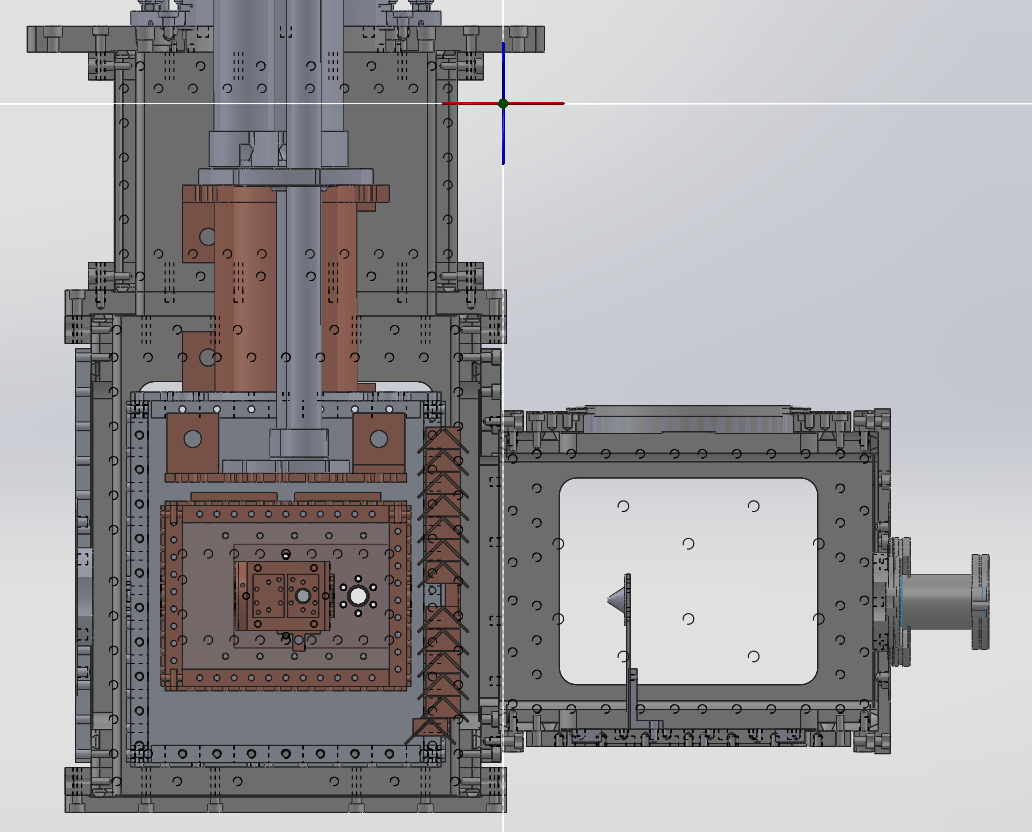
\includegraphics[width=1\textwidth]{images/CBGB_solidworks_cross_section.png}
	\caption{Cross sectional view of CBGB in solidworks. Components include copper sheath for PTR, aluminum radiation shield with chevron baffles, copper shield and experimental cell, and skimmer mounted in stem chamber. The baffles allow for gas to flow into the cold region of the beam apparatus, while preventing 300K black body radiation from hitting the inner shield and cell.}
	\label{fig: SW chamber}
\end{figure}

The mounting of the inner components was of particular importance due to the fragility of the PTR as well as the desire to minimize thermal conductivity to the experimental region. All the shield components were mounted to the top mounting plate 

\todo{solidworks image of system}

\begin{figure}[H]
	\centering
	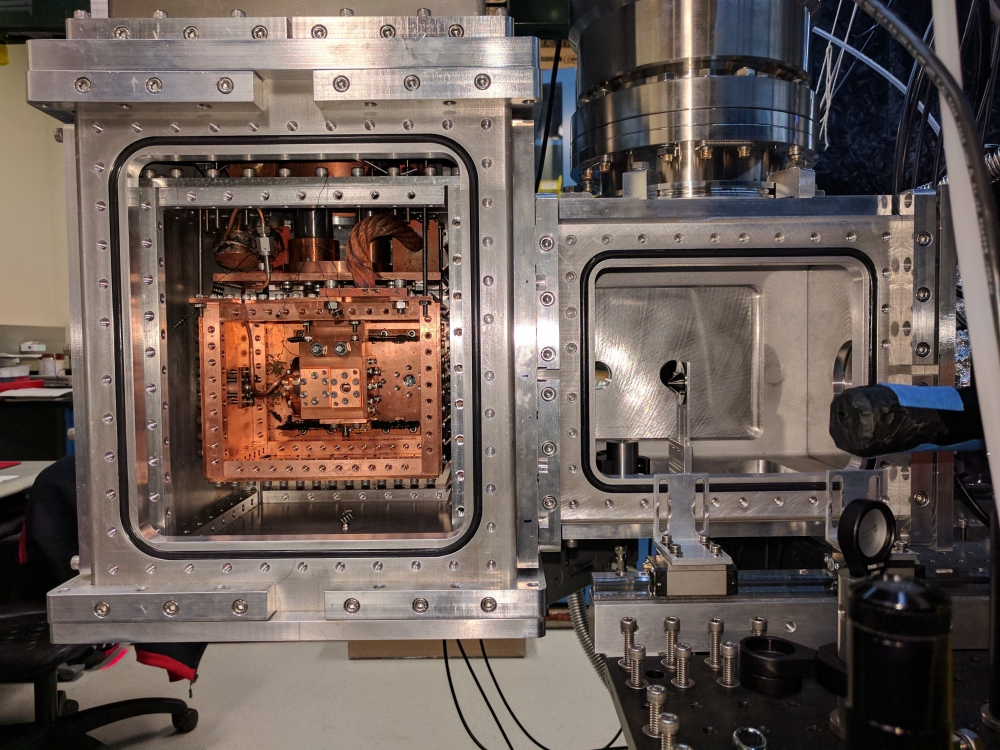
\includegraphics[width=1\textwidth]{images/CBGB_cross_section.jpg}
	\caption{Cross sectional view of CBGB with side walls removed from the outer vacuum chamber, 40K aluminum radiation shield, and inner 4K cryopumping shield exposing the inner experimental cell. A skimmer is mounted in the stem region.}
	\label{fig: chamber}
\end{figure}

\begin{figure}[H]
	\centering
	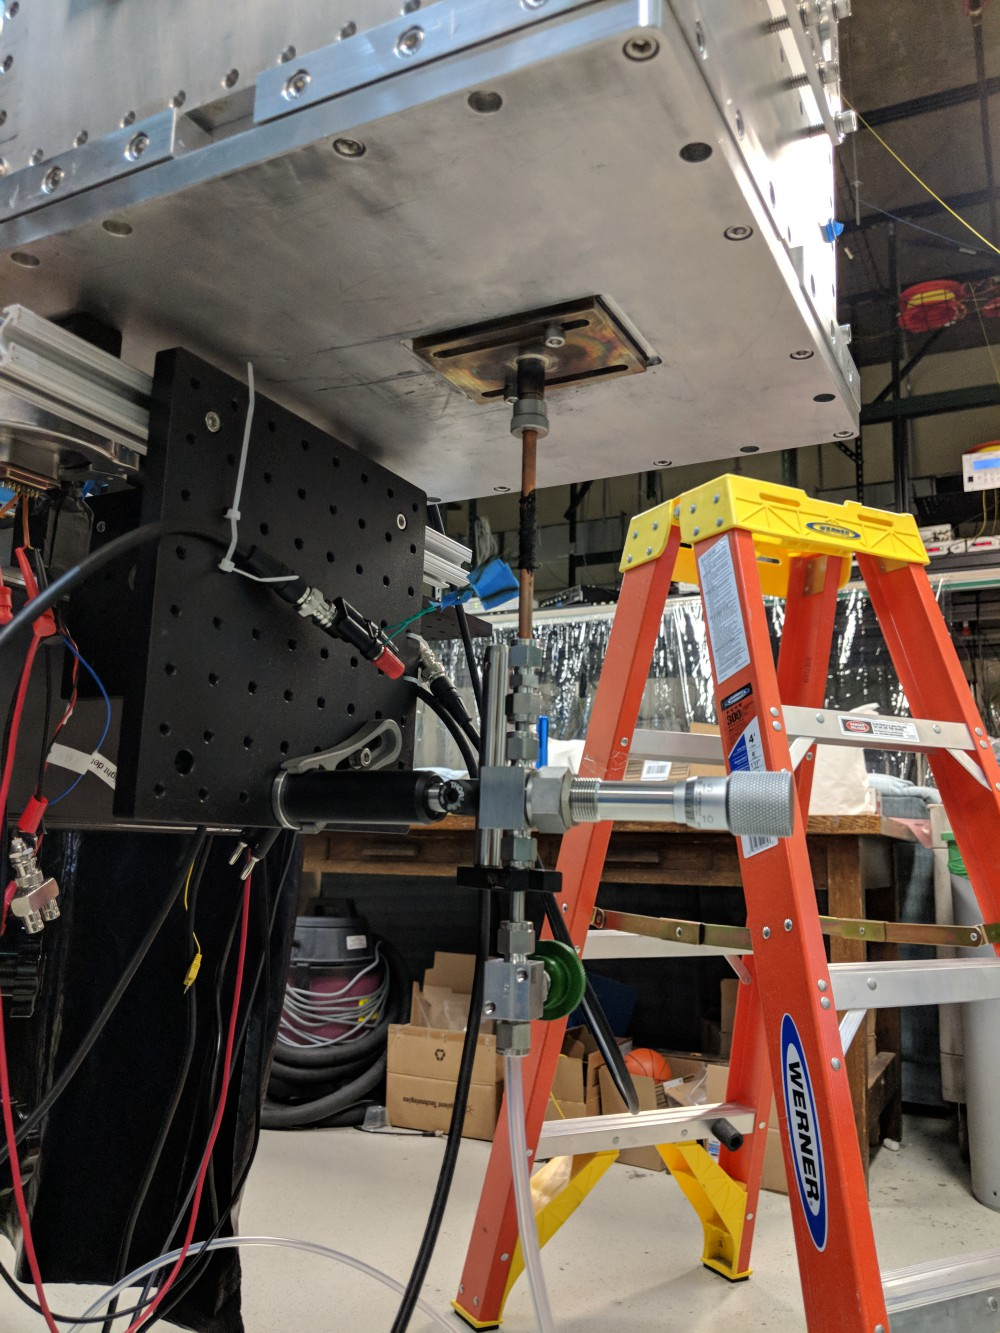
\includegraphics[width=.7\textwidth]{images/CBGB_water_fill_outside.jpg}
	\caption{The water fill line, sealed by an ultratorr fitting and heated by nichrome wire. A shut off valve and vernier valve are used to regulate the flow of water into the buffer gas cell.}
	\label{fig: outside}
\end{figure}

\begin{figure}[H]
	\centering
	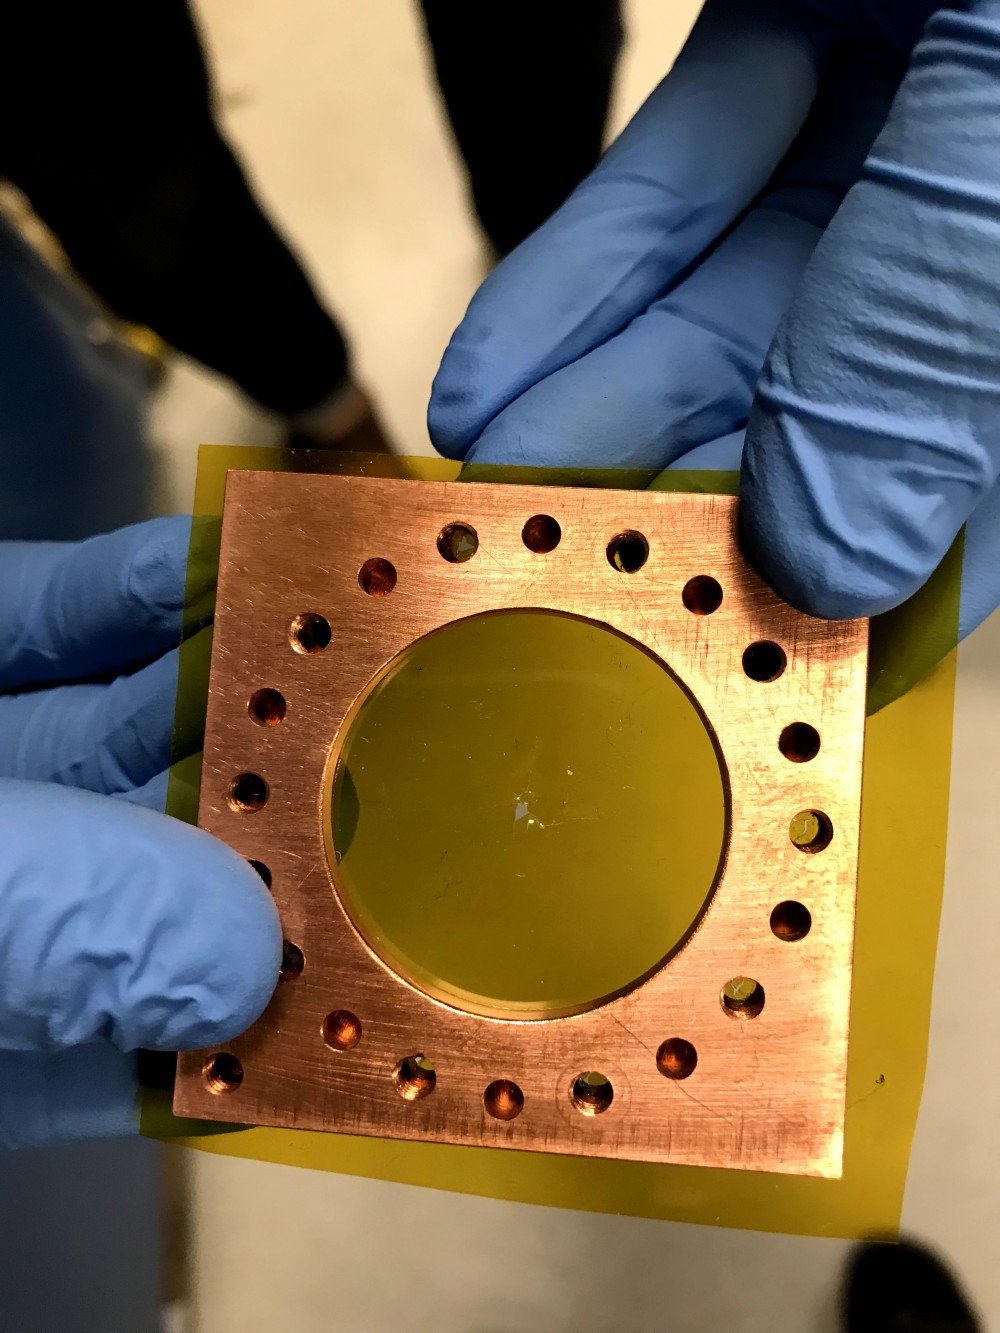
\includegraphics[width=.7\textwidth]{images/CBGB_kapton.jpg}
	\caption{A kapton film serves as the back wall of the buffer gas cell with a hole for the insertion of the water fill line. The kapton surface resists ice formation and allows for continuous operation with water for over 10 hours.}
	\label{fig: kapton}
\end{figure}